\documentclass[exercice]{thedocument}%
\usepackage{tikz}
\usepackage{texmaths-symbols}
\startdatakeys
\source{}
\cycle{}
\competencesDuSocle{}
\connaissancesRequises{}
\competencesTravaillees{}
\enddatakeys
\begin{document}%
\begin{minipage}[t]{.5\linewidth}
    \begin{enumerate}
        \item Dans le cahier, placer six points comme ci-contre.
        \item Dans chaque cas, écrire avec les notations mathématiques
        et compléter la figure.
        \begin{enumerate}
            \item Le semgent d'extrémités les points A et B.
            \item La droite passant par les points C et D.
            \item La demi-droite d'origine B passant par E.
        \end{enumerate}
    \end{enumerate}
\end{minipage}\hskip20pt minus 10pt
    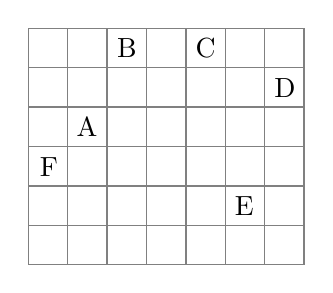
\begin{tikzpicture}[scale=0.5, baseline=(current bounding box.north)]
        \coordinate[label=above left:A](A)at(2,3);
        \coordinate[label=above left:B](B)at(3,5);
        \coordinate[label=above right:C](C)at(4,5);
        \coordinate[label=above right:D](D)at(6,4);
        \coordinate[label=above right:E](E)at(5,1);
        \coordinate[label=above left:F](F)at(1,2);
        \draw[line width=0.5pt,gray] (0,0)grid(7,6);
        \draw node at (A){\cross};
        \draw node at (B){\cross};
        \draw node at (C){\cross};
        \draw node at (D){\cross};
        \draw node at (E){\cross};
        \draw node at (F){\cross};
    \end{tikzpicture}
\end{document}
